%% V1.4a
%% 2014/09/17
%% by Michael Shell
%% see http://www.michaelshell.org/
%% for current contact information.
%%
%% This is a skeleton file demonstrating the use of IEEEtran.cls
%% (requires IEEEtran.cls version 1.8a or later) with an IEEE
%% journal paper.
%%
%% Support sites:
%% http://www.michaelshell.org/tex/ieeetran/
%% http://www.ctan.org/tex-archive/macros/latex/contrib/IEEEtran/
%% and
%% http://www.ieee.org/

%%*************************************************************************
%% Legal Notice:
%% This code is offered as-is without any warranty either expressed or
%% implied; without even the implied warranty of MERCHANTABILITY or
%% FITNESS FOR A PARTICULAR PURPOSE! 
%% User assumes all risk.
%% In no event shall IEEE or any contributor to this code be liable for
%% any damages or losses, including, but not limited to, incidental,
%% consequential, or any other damages, resulting from the use or misuse
%% of any information contained here.
%%
%% All comments are the opinions of their respective authors and are not
%% necessarily endorsed by the IEEE.
%%
%% This work is distributed under the LaTeX Project Public License (LPPL)
%% ( http://www.latex-project.org/ ) version 1.3, and may be freely used,
%% distributed and modified. A copy of the LPPL, version 1.3, is included
%% in the base LaTeX documentation of all distributions of LaTeX released
%% 2003/12/01 or later.
%% Retain all contribution notices and credits.
%% ** Modified files should be clearly indicated as such, including  **
%% ** renaming them and changing author support contact information. **
%%
%% File list of work: IEEEtran.cls, IEEEtran_HOWTO.pdf, bare_adv.tex,
%%                    bare_conf.tex, bare_jrnl.tex, bare_conf_compsoc.tex,
%%                    bare_jrnl_compsoc.tex, bare_jrnl_transmag.tex
%%*************************************************************************


% *** Authors should verify (and, if needed, correct) their LaTeX system  ***
% *** with the testflow diagnostic prior to trusting their LaTeX platform ***
% *** with production work. IEEE's font choices and paper sizes can       ***
% *** trigger bugs that do not appear when using other class files.       ***                          ***
% The testflow support page is at:
% http://www.michaelshell.org/tex/testflow/



\documentclass[10pt, journal,twocolumn]{IEEEtran}
%
% If IEEEtran.cls has not been installed into the LaTeX system files,
% manually specify the path to it like:
% \documentclass[journal]{../sty/IEEEtran}



\usepackage[utf8]{inputenc}
\usepackage[italian]{babel}

\usepackage{amsmath}
\usepackage{amsfonts}
\usepackage{amssymb}
\usepackage{amsthm}

\usepackage{graphicx}
\usepackage{subcaption}

% \setlength{\columnseprule}{0,1mm}




% Some very useful LaTeX packages include:
% (uncomment the ones you want to load)


% *** MISC UTILITY PACKAGES ***
%
%\usepackage{ifpdf}
% Heiko Oberdiek's ifpdf.sty is very useful if you need conditional
% compilation based on whether the output is pdf or dvi.
% usage:
% \ifpdf
%   % pdf code
% \else
%   % dvi code
% \fi
% The latest version of ifpdf.sty can be obtained from:
% http://www.ctan.org/tex-archive/macros/latex/contrib/oberdiek/
% Also, note that IEEEtran.cls V1.7 and later provides a builtin
% \ifCLASSINFOpdf conditional that works the same way.
% When switching from latex to pdflatex and vice-versa, the compiler may
% have to be run twice to clear warning/error messages.






% *** CITATION PACKAGES ***
%
%\usepackage{cite}
% cite.sty was written by Donald Arseneau
% V1.6 and later of IEEEtran pre-defines the format of the cite.sty package
% \cite{} output to follow that of IEEE. Loading the cite package will
% result in citation numbers being automatically sorted and properly
% "compressed/ranged". e.g., [1], [9], [2], [7], [5], [6] without using
% cite.sty will become [1], [2], [5]--[7], [9] using cite.sty. cite.sty's
% \cite will automatically add leading space, if needed. Use cite.sty's
% noadjust option (cite.sty V3.8 and later) if you want to turn this off
% such as if a citation ever needs to be enclosed in parenthesis.
% cite.sty is already installed on most LaTeX systems. Be sure and use
% version 5.0 (2009-03-20) and later if using hyperref.sty.
% The latest version can be obtained at:
% http://www.ctan.org/tex-archive/macros/latex/contrib/cite/
% The documentation is contained in the cite.sty file itself.






% *** GRAPHICS RELATED PACKAGES ***
%
\ifCLASSINFOpdf
  % \usepackage[pdftex]{graphicx}
  % declare the path(s) where your graphic files are
  % \graphicspath{{../pdf/}{../jpeg/}}
  % and their extensions so you won't have to specify these with
  % every instance of \includegraphics
  % \DeclareGraphicsExtensions{.pdf,.jpeg,.png}
\else
  % or other class option (dvipsone, dvipdf, if not using dvips). graphicx
  % will default to the driver specified in the system graphics.cfg if no
  % driver is specified.
  % \usepackage[dvips]{graphicx}
  % declare the path(s) where your graphic files are
  % \graphicspath{{../eps/}}
  % and their extensions so you won't have to specify these with
  % every instance of \includegraphics
  % \DeclareGraphicsExtensions{.eps}
\fi
% graphicx was written by David Carlisle and Sebastian Rahtz. It is
% required if you want graphics, photos, etc. graphicx.sty is already
% installed on most LaTeX systems. The latest version and documentation
% can be obtained at: 
% http://www.ctan.org/tex-archive/macros/latex/required/graphics/
% Another good source of documentation is "Using Imported Graphics in
% LaTeX2e" by Keith Reckdahl which can be found at:
% http://www.ctan.org/tex-archive/info/epslatex/
%
% latex, and pdflatex in dvi mode, support graphics in encapsulated
% postscript (.eps) format. pdflatex in pdf mode supports graphics
% in .pdf, .jpeg, .png and .mps (metapost) formats. Users should ensure
% that all non-photo figures use a vector format (.eps, .pdf, .mps) and
% not a bitmapped formats (.jpeg, .png). IEEE frowns on bitmapped formats
% which can result in "jaggedy"/blurry rendering of lines and letters as
% well as large increases in file sizes.
%
% You can find documentation about the pdfTeX application at:
% http://www.tug.org/applications/pdftex





% *** MATH PACKAGES ***
%
\usepackage{amsmath} 
\usepackage{amsopn} 
% \usepackage[cmex10]{amsmath}
% A popular package from the American Mathematical Society that provides
% many useful and powerful commands for dealing with mathematics. If using
% it, be sure to load this package with the cmex10 option to ensure that
% only type 1 fonts will utilized at all point sizes. Without this option,
% it is possible that some math symbols, particularly those within
% footnotes, will be rendered in bitmap form which will result in a
% document that can not be IEEE Xplore compliant!
%
% Also, note that the amsmath package sets \interdisplaylinepenalty to 10000
% thus preventing page breaks from occurring within multiline equations. Use:
% \interdisplaylinepenalty=2500
% after loading amsmath to restore such page breaks as IEEEtran.cls normally
% does. amsmath.sty is already installed on most LaTeX systems. The latest
% version and documentation can be obtained at:
% http://www.ctan.org/tex-archive/macros/latex/required/amslatex/math/


\DeclareMathOperator{\mtdt}{metadata} 
\DeclareMathOperator{\distn}{dNews}
\DeclareMathOperator{\disti}{dImg}



% *** SPECIALIZED LIST PACKAGES ***
%
\usepackage{algorithmic}
% algorithmic.sty was written by Peter Williams and Rogerio Brito.
% This package provides an algorithmic environment fo describing algorithms.
% You can use the algorithmic environment in-text or within a figure
% environment to provide for a floating algorithm. Do NOT use the algorithm
% floating environment provided by algorithm.sty (by the same authors) or
% algorithm2e.sty (by Christophe Fiorio) as IEEE does not use dedicated
% algorithm float types and packages that provide these will not provide
% correct IEEE style captions. The latest version and documentation of
% algorithmic.sty can be obtained at:
% http://www.ctan.org/tex-archive/macros/latex/contrib/algorithms/
% There is also a support site at:
% http://algorithms.berlios.de/index.html
% Also of interest may be the (relatively newer and more customizable)
% algorithmicx.sty package by Szasz Janos:
% http://www.ctan.org/tex-archive/macros/latex/contrib/algorithmicx/




% *** ALIGNMENT PACKAGES ***
%
\usepackage{array}
% Frank Mittelbach's and David Carlisle's array.sty patches and improves
% the standard LaTeX2e array and tabular environments to provide better
% appearance and additional user controls. As the default LaTeX2e table
% generation code is lacking to the point of almost being broken with
% respect to the quality of the end results, all users are strongly
% advised to use an enhanced (at the very least that provided by array.sty)
% set of table tools. array.sty is already installed on most systems. The
% latest version and documentation can be obtained at:
% http://www.ctan.org/tex-archive/macros/latex/required/tools/


% IEEEtran contains the IEEEeqnarray family of commands that can be used to
% generate multiline equations as well as matrices, tables, etc., of high
% quality.




% *** SUBFIGURE PACKAGES ***
%\ifCLASSOPTIONcompsoc
%  \usepackage[caption=false,font=normalsize,labelfont=sf,textfont=sf]{subfig}
%\else
%  \usepackage[caption=false,font=footnotesize]{subfig}
%\fi
% subfig.sty, written by Steven Douglas Cochran, is the modern replacement
% for subfigure.sty, the latter of which is no longer maintained and is
% incompatible with some LaTeX packages including fixltx2e. However,
% subfig.sty requires and automatically loads Axel Sommerfeldt's caption.sty
% which will override IEEEtran.cls' handling of captions and this will result
% in non-IEEE style figure/table captions. To prevent this problem, be sure
% and invoke subfig.sty's "caption=false" package option (available since
% subfig.sty version 1.3, 2005/06/28) as this is will preserve IEEEtran.cls
% handling of captions.
% Note that the Computer Society format requires a larger sans serif font
% than the serif footnote size font used in traditional IEEE formatting
% and thus the need to invoke different subfig.sty package options depending
% on whether compsoc mode has been enabled.
%
% The latest version and documentation of subfig.sty can be obtained at:
% http://www.ctan.org/tex-archive/macros/latex/contrib/subfig/




% *** FLOAT PACKAGES ***
%
%\usepackage{fixltx2e}
% fixltx2e, the successor to the earlier fix2col.sty, was written by
% Frank Mittelbach and David Carlisle. This package corrects a few problems
% in the LaTeX2e kernel, the most notable of which is that in current
% LaTeX2e releases, the ordering of single and double column floats is not
% guaranteed to be preserved. Thus, an unpatched LaTeX2e can allow a
% single column figure to be placed prior to an earlier double column
% figure. The latest version and documentation can be found at:
% http://www.ctan.org/tex-archive/macros/latex/base/


%\usepackage{stfloats}
% stfloats.sty was written by Sigitas Tolusis. This package gives LaTeX2e
% the ability to do double column floats at the bottom of the page as well
% as the top. (e.g., "\begin{figure*}[!b]" is not normally possible in
% LaTeX2e). It also provides a command:
%\fnbelowfloat
% to enable the placement of footnotes below bottom floats (the standard
% LaTeX2e kernel puts them above bottom floats). This is an invasive package
% which rewrites many portions of the LaTeX2e float routines. It may not work
% with other packages that modify the LaTeX2e float routines. The latest
% version and documentation can be obtained at:
% http://www.ctan.org/tex-archive/macros/latex/contrib/sttools/
% Do not use the stfloats baselinefloat ability as IEEE does not allow
% \baselineskip to stretch. Authors submitting work to the IEEE should note
% that IEEE rarely uses double column equations and that authors should try
% to avoid such use. Do not be tempted to use the cuted.sty or midfloat.sty
% packages (also by Sigitas Tolusis) as IEEE does not format its papers in
% such ways.
% Do not attempt to use stfloats with fixltx2e as they are incompatible.
% Instead, use Morten Hogholm'a dblfloatfix which combines the features
% of both fixltx2e and stfloats:
%
% \usepackage{dblfloatfix}
% The latest version can be found at:
% http://www.ctan.org/tex-archive/macros/latex/contrib/dblfloatfix/




%\ifCLASSOPTIONcaptionsoff
%  \usepackage[nomarkers]{endfloat}
% \let\MYoriglatexcaption\caption
% \renewcommand{\caption}[2][\relax]{\MYoriglatexcaption[#2]{#2}}
%\fi
% endfloat.sty was written by James Darrell McCauley, Jeff Goldberg and 
% Axel Sommerfeldt. This package may be useful when used in conjunction with 
% IEEEtran.cls'  captionsoff option. Some IEEE journals/societies require that
% submissions have lists of figures/tables at the end of the paper and that
% figures/tables without any captions are placed on a page by themselves at
% the end of the document. If needed, the draftcls IEEEtran class option or
% \CLASSINPUTbaselinestretch interface can be used to increase the line
% spacing as well. Be sure and use the nomarkers option of endfloat to
% prevent endfloat from "marking" where the figures would have been placed
% in the text. The two hack lines of code above are a slight modification of
% that suggested by in the endfloat docs (section 8.4.1) to ensure that
% the full captions always appear in the list of figures/tables - even if
% the user used the short optional argument of \caption[]{}.
% IEEE papers do not typically make use of \caption[]'s optional argument,
% so this should not be an issue. A similar trick can be used to disable
% captions of packages such as subfig.sty that lack options to turn off
% the subcaptions:
% For subfig.sty:
% \let\MYorigsubfloat\subfloat
% \renewcommand{\subfloat}[2][\relax]{\MYorigsubfloat[]{#2}}
% However, the above trick will not work if both optional arguments of
% the \subfloat command are used. Furthermore, there needs to be a
% description of each subfigure *somewhere* and endfloat does not add
% subfigure captions to its list of figures. Thus, the best approach is to
% avoid the use of subfigure captions (many IEEE journals avoid them anyway)
% and instead reference/explain all the subfigures within the main caption.
% The latest version of endfloat.sty and its documentation can obtained at:
% http://www.ctan.org/tex-archive/macros/latex/contrib/endfloat/
%
% The IEEEtran \ifCLASSOPTIONcaptionsoff conditional can also be used
% later in the document, say, to conditionally put the References on a 
% page by themselves.




% *** PDF, URL AND HYPERLINK PACKAGES ***
%
\usepackage{url}
% url.sty was written by Donald Arseneau. It provides better support for
% handling and breaking URLs. url.sty is already installed on most LaTeX
% systems. The latest version and documentation can be obtained at:
% http://www.ctan.org/tex-archive/macros/latex/contrib/url/
% Basically, \url{my_url_here}.




% *** Do not adjust lengths that control margins, column widths, etc. ***
% *** Do not use packages that alter fonts (such as pslatex).         ***
% There should be no need to do such things with IEEEtran.cls V1.6 and later.
% (Unless specifically asked to do so by the journal or conference you plan
% to submit to, of course. )


% correct bad hyphenation here



\begin{document}
%
% paper title
% Titles are generally capitalized except for words such as a, an, and, as,
% at, but, by, for, in, nor, of, on, or, the, to and up, which are usually
% not capitalized unless they are the first or last word of the title.
% Linebreaks \\ can be used within to get better formatting as desired.
% Do not put math or special symbols in the title.
\title{An empiric way to media discrimination in news}
%
%
% author names and IEEE memberships
% note positions of commas and nonbreaking spaces ( ~ ) LaTeX will not break
% a structure at a ~ so this keeps an author's name from being broken across
% two lines.
% use \thanks{} to gain access to the first footnote area
% a separate \thanks must be used for each paragraph as LaTeX2e's \thanks
% was not built to handle multiple paragraphs
%

\author{Carlo~Brunetta,
        Andrea~Vinci, etc}% <-this % stops a space
% \thanks{M. Shell is with the Department
% of Electrical and Computer Engineering, Georgia Institute of Technology, Atlanta,
% GA, 30332 USA e-mail: (see http://www.michaelshell.org/contact.html).}% <-this % stops a space
% \thanks{J. Doe and J. Doe are with Anonymous University.}% <-this % stops a space
% \thanks{Manuscript received April 19, 2005; revised September 17, 2014.}}

% note the % following the last \IEEEmembership and also \thanks - 
% these prevent an unwanted space from occurring between the last author name
% and the end of the author line. i.e., if you had this:
% 
% \author{....lastname \thanks{...} \thanks{...} }
%                     ^------------^------------^----Do not want these spaces!
%
% a space would be appended to the last name and could cause every name on that
% line to be shifted left slightly. This is one of those "LaTeX things". For
% instance, "\textbf{A} \textbf{B}" will typeset as "A B" not "AB". To get
% "AB" then you have to do: "\textbf{A}\textbf{B}"
% \thanks is no different in this regard, so shield the last } of each \thanks
% that ends a line with a % and do not let a space in before the next \thanks.
% Spaces after \IEEEmembership other than the last one are OK (and needed) as
% you are supposed to have spaces between the names. For what it is worth,
% this is a minor point as most people would not even notice if the said evil
% space somehow managed to creep in.



% The paper headers
\markboth{Something}{}%

% The only time the second header will appear is for the odd numbered pages
% after the title page when using the twoside option.
% 
% *** Note that you probably will NOT want to include the author's ***
% *** name in the headers of peer review papers.                   ***
% You can use \ifCLASSOPTIONpeerreview for conditional compilation here if
% you desire.




% If you want to put a publisher's ID mark on the page you can do it like
% this:
%\IEEEpubid{0000--0000/00\$00.00~\copyright~2014 IEEE}
% Remember, if you use this you must call \IEEEpubidadjcol in the second
% column for its text to clear the IEEEpubid mark.



% use for special paper notices
%\IEEEspecialpapernotice{(Invited Paper)}




% make the title area
\maketitle

% As a general rule, do not put math, special symbols or citations
% in the abstract or keywords.
\begin{abstract}
With this paper we want to analyze the problem of image discrimination related to a news that can be found on the Internet. Our goal is to create an empirical way to 
see if the image is related with the news even in a semantic meaning and in a temporal view.
\end{abstract}

% Note that keywords are not normally used for peerreview papers.
\begin{IEEEkeywords}
Key, key, key
\end{IEEEkeywords}






% For peer review papers, you can put extra information on the cover
% page as needed:
% \ifCLASSOPTIONpeerreview
% \begin{center} \bfseries EDICS Category: 3-BBND \end{center}
% \fi
%
% For peerreview papers, this IEEEtran command inserts a page break and
% creates the second title. It will be ignored for other modes.
\IEEEpeerreviewmaketitle



\section{Introduction}
% The very first letter is a 2 line initial drop letter followed
% by the rest of the first word in caps.
% 
% form to use if the first word consists of a single letter:
% \IEEEPARstart{A}{demo} file is ....
% 
% form to use if you need the single drop letter followed by
% normal text (unknown if ever used by IEEE):
% \IEEEPARstart{A}{}demo file is ....
% 
% Some journals put the first two words in caps:
% \IEEEPARstart{T}{his demo} file is ....
% 
% Here we have the typical use of a "T" for an initial drop letter
% and "HIS" in caps to complete the first word.
\IEEEPARstart{W}{ith} the increasing information that can be found on the Internet, is hard to trace and believe if a news website can be trust.\\
In this framework is really hard to define if ``an image is related with the news''. We can have that the news is real but the image is decontestualized because it could, for example, be taken in another time period or has been tampered.\\
So we investigate a way to check if a given news has coerent image with respect to the content of the news without using any authorative database. We will try to define some ``metadata'' that will be used to analyze the correctness of the (news,image) couple.
% You must have at least 2 lines in the paragraph with the drop letter
% (should never be an issue)
 
\hfill Month, Day Year

\subsection{Math legend}
\begin{itemize}
	\item $\mathcal{N}$ : the set of all the news
	\item $\mathcal{M}$ : the set of all the metadata
	\item $\mathcal{I}$ : the set of all the images
\end{itemize}

\subsection{Main idea}


To analyze the single news $N$ we want to extract some metadata $\mu_N$ that describe and discriminate the news $N$.\\
We define a function $\mtdt : \mathcal{N} \rightarrow \mathcal{M} \times \mathcal{I}$ that $\mtdt(N) = (\mu_N , \xi_N)$ where $\mu_x$ will contain 
\begin{itemize}
 	\item Title of the news
 	\item Body
 	\item \textbf{Date}
 	\item Tags of the news \label{tags1}
\end{itemize} 
and $\xi_N$ will just be the set of the images contained in $N$.\\[0,1cm]

The ``tags''-metadata is critical. We want to obtain some keywords that can describe the contest of the news. We assume that from these keywords we can understand the sector of the news.\\
The usage of the tags is critical for the discrimination of $N$.

We can see the ``title'' as a real precise metadata that will always descrive the same event. The ``tags'' will create \emph{noise} in the possible event description so if we analyze it we can optain really temporal-different news but with the same semantic meaning.\\[0,3cm]

We define the set $G_N$ as the set of news that has a similar title with respect to a given threshold $\tau_1$.\\
Then we define $G_N^\prime$ as the set of news with similar tag with respect to the threshold $\tau_1$.\\
We now define $\mathcal{G}_N := \{ f(G_N,G_N^\prime) \} \subseteq \mathcal{N}$ as a subset of all the news that has some correlation in the title \textbf{and} in the description.\\
In this way we have empirically done a characterization of the news and extracted just the news that have a high correlation in the metadata.\\[0,2cm]

We now define for every $N \in \mathcal{N}$ and for every $M \in \mathcal{M}$  the distance $\distn_N(M)$ that measure ``the metadata distance'' of $M$ with respect to $N$.\\
In the same way, we define a measure $\disti_N(M)$ that measure the ``image distance'' between the images of two news.\\[0.3cm]


So, from a given news $N$, we do:

\begin{enumerate}
	\item $\mtdt(N) = (\mu_N,\xi_N)$
	\item Construct $\mathcal{G}_N$
	\item Search, with a given threshold $\tau_1$, all the metadata-close news $H \subset \mathcal{G}_N$
	\item Search, with a given threshold $\tau_2$, all the image-close news $J \subset \mathcal{G}_N$
\end{enumerate}

\-\\[0,1cm]

At this point we can introduce some empiric ideas:

\begin{center}
\emph{If a news $M \in H$ and $\exists O \in J$ such that $\xi_M \cap \xi_O \neq \emptyset$ then an image of $N$ is likely to be coherent with the metadata.}
\end{center}

If a news is metadata-close to $N$ and has some images $\xi$ that is image-close, then we have $\xi$ as a particular image that is likely to be coherent with the news.\\[0.2cm]

\begin{center}
\emph{If a news $M \in J$ has $\distn_N(M) < \tau_1$ then is likely that the image is not correlated with the news.}
\end{center}

A image-close news but with not near metadata-distance assure that $N$ is probably incoherent.\\[0.2cm]

\begin{center}
\emph{If a news $M \in J \cap H$ but the ``date''-metadata is not close, then one of the two news has a incoherent use of image-news.} \label{terzocaso}
\end{center}

A news near in metadata and image distances but with different date will imply that there's a incoherence in one of the two news.\\[0.2cm]


With these empiric rules, we can create a distinguisher to distinguish if a news image is coherent with the news metadata.\\[0.1cm]

In this mathematical description, we work with sets of \emph{``all the possible $x$''}.\\
In our implementation we increase the distinguisher capacity by applying the empiric rules in a really bigger set. For example, if we have two news from the third rule, we can check the two news to see which of the three is the real incoherent news.\\
Notice that we don't assume if the news are real or not but just want to control the coherence of a single news.



\section{Implementation}

Because is really hard to retrive the set $\mathcal{G}$, we assume and use Google as the search motor to retrive all the set of our scheme.\\
In the same way is impossible to achieve the sets $G_N$ and $G_N^\prime$ because of their size so we will restrict the search in a smaller set of result. The conseguence is that we will operate with a different $\overline{\mathcal{G}}_N$ that will just be the \emph{Top 10} of $G_N$ and the \emph{Top 10} of $G^\prime_N$.\\[0.2cm]

To implement our schema, we used Python 3.4 and Matlab.\\
The workflow is divided in this step:
\begin{itemize}
  \item \textbf{Downloading Phase} : from a news link we download all the correlated news via the title and the tags. All these (metadata,image) are inserted into a database.
  \item \textbf{Similar Analysis} : we concentrate on the image and using similarity algorithms, we filla table in the database.
  \item \textbf{Check Data} : we can procede in two way:
  \begin{itemize}
    \item \textbf{Human-like} : we check if the images are similar using a simple interface
    \item \textbf{Threshold-like} : we automatize the analisis by valuating the values of the parameter we have with a given threshold
  \end{itemize}
\end{itemize}


\subsection{Downloading Phase}

From a link to a news, using Python and module that can be found on github, we extrapolate all the metadata of the original news and the correlated ones.\\[0,2cm]

We divided the work in three main modules:
\begin{itemize}
  \item \textbf{NewsParser} : using \emph{newspaper}\footnote{link} we parse the original news and get all the metadata except for the \emph{tags}-metadata. These tags are created by a simple \emph{tagger} we create using \emph{ntlk}.\\
  \textbf{Input : } url of a news\\
  \textbf{Output : } json with all the metadata
  \item \textbf{GoogleSearcher} : using \emph{GoogleScrapper}\footnote{link} we search on Google a choosen string.
  \textbf{Input : } string to search\\
  \textbf{Output : } list of the first result
  \item \textbf{DBManager : } using \emph{sqlite3} we create the database with all the metadata and images of the news.\\
  \textbf{Input : } newses jsons\\
  \textbf{Output : } database with all the information 
\end{itemize}

These three module have this workflow:

\begin{enumerate}
  \item From the original link, we apply NewsParser and obtain the complete description with (metadata,images)
  \item We search owith GoogleSearcher using as string the \emph{title}-metadata and \emph{tags}-metadata.
  \item All the result are parsed with NewsParser
  \item All the information are saved with DBManager into a database
\end{enumerate}


\subsection{Similar Analysis}

Using MATLAB, we measure the similarity using \emph{SURF} and the \emph{correlation}.\\
We calculate all the value between a single image of the original news with all the images founded by the reserch.\\[0,1cm]
All these value are saved in the database.

\subsection{Check Data}

\subsubsection{Human-like}

We create, using XCode, an interface where all the similarity are shown one after the other.\\
The user is asked to answer \emph{``are the two images correlated?''}.\\[0,1cm]
In this way, from the database, we can check all the similar image and obtain:
\begin{itemize}
  \item Threshold for that particular image
  \item \emph{Data}-metadata analisys for discriminating over the time
\end{itemize}

With these operation, if we are lucky enough to have some similarity in the researched images, we can answer \emph{``is the original image coherent with the news?''} or \emph{``is there some strange behaviour of the image?''}

\subsubsection{Threshold-like}

From the database, we can automatically check the value of \emph{SURF} and \emph{corelation} and, given a function $f(\tau_{\text{SURF}} , \tau_{\text{cor}})$, filter the similar images.\\
From these we can analyse the \emph{data}-metadata and see if there is a strange behaviour.\\
With a high value of threshold, we suppose that we can answer to \emph{``is the original image coherent with the news?''} .


\section{Testing}

We operate with three type of test:

\begin{enumerate}
  \item \textbf{Human-like only} : statistically analyse \emph{how} we can choose the threshold given by the function $f(\tau_{\text{SURF}} , \tau_{\text{cor}})$.
  \item \textbf{Threshold-like only} : analyse the behaviour of the coherence-analyser trying different threshold functions.
  \item \textbf{Human-Threshold check} : we operate with the same news with all the two test and trace conclusion on the efficency of the scheme.
\end{enumerate}

\subsection{Human-like only}

Considerated the consisted number of similarity to manually check ($\sim 2000$ order), we tested the scheme in a Human-like Check Data, with three news:

\begin{enumerate}
  \item \textbf{BBC} - \emph{Charlie Hebdo attack: Three days of terror} \footnote{\url{http://www.bbc.com/news/world-europe-30708237}}
  \item \textbf{MailOnline} - \emph{ISIS knew burning Jordanian pilot alive would spark backlash in Islamic world - so prepared a list of justifications beforehand} \footnote{\url{http://www.dailymail.co.uk/news/article-2938886/}}
  \item \textbf{NBC} - \emph{Turkish Airlines Jet Skids Off Foggy Runway in Kathmandu, Nepal} \footnote{\url{http://www.nbcnews.com/news/world/turkish-airlines-jet-skids-foggy-runway-kathmandu-nepal-n316956}}
  \item \textbf{BBC} - \emph{Russia opposition politician Boris Nemtsov shot dead} \footnote{http://www.bbc.com/news/world-europe-31669061}
\end{enumerate}

After the Check Data, we get these results :

\begin{center}
\begin{tabular}{|c|c|c|}
\hline
Test Number & \# Total images & \# Similar images \\
\hline\hline
1 & $5616$ & $81$ \\    \hline
2 & $1010$ & $32$ \\    \hline
3 & $55$ & $6$    \\ \hline
4 & $1064$ & $23$ \\ \hline
\end{tabular}
\end{center}

From the manual classification, we plotted a rappresentation on the plan (\emph{SURF} value $\times$ Correlation) where the red dots will classify the similar images and the blu the non similar ones. We excluded the images with the same url because these have a fixed $(1.0 , 1.0)$ coordinate.\\

\begin{figure}[!ht]
\begin{subfigure}{.25\textwidth}
  \begin{center}
  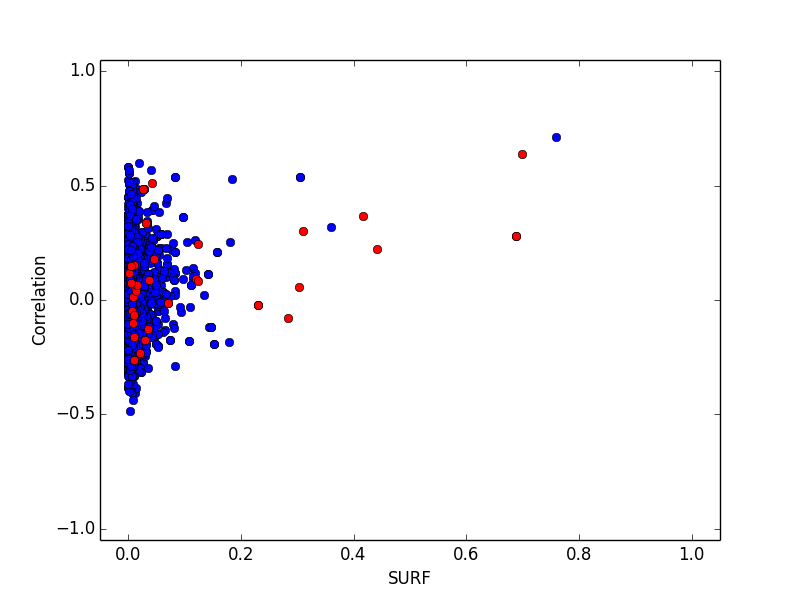
\includegraphics[keepaspectratio,width=1\textwidth]{1}\\
{News 1}
  \end{center}
\end{subfigure}%
\begin{subfigure}{.25\textwidth}
  \begin{center}
  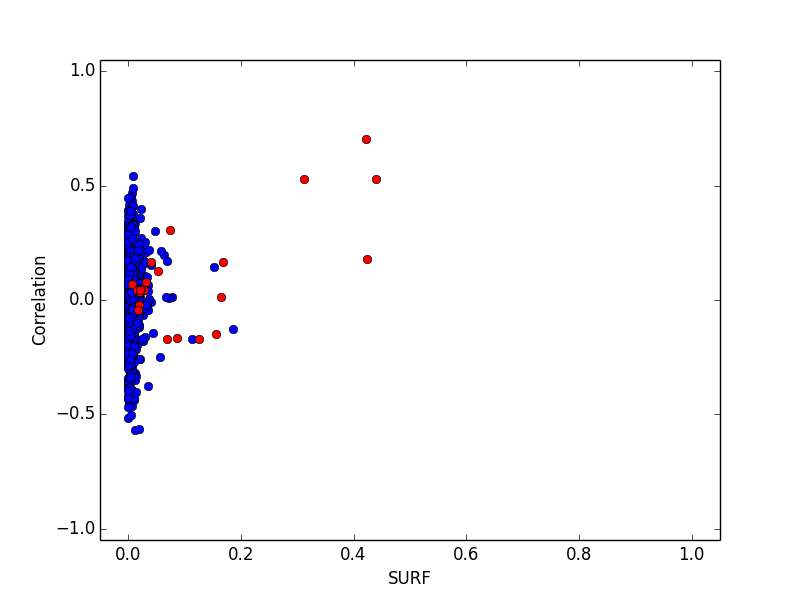
\includegraphics[keepaspectratio,width=1\textwidth]{2}\\
{News 2}
  \end{center}
\end{subfigure}
\-\\
\begin{subfigure}{.25\textwidth}
  \begin{center}
  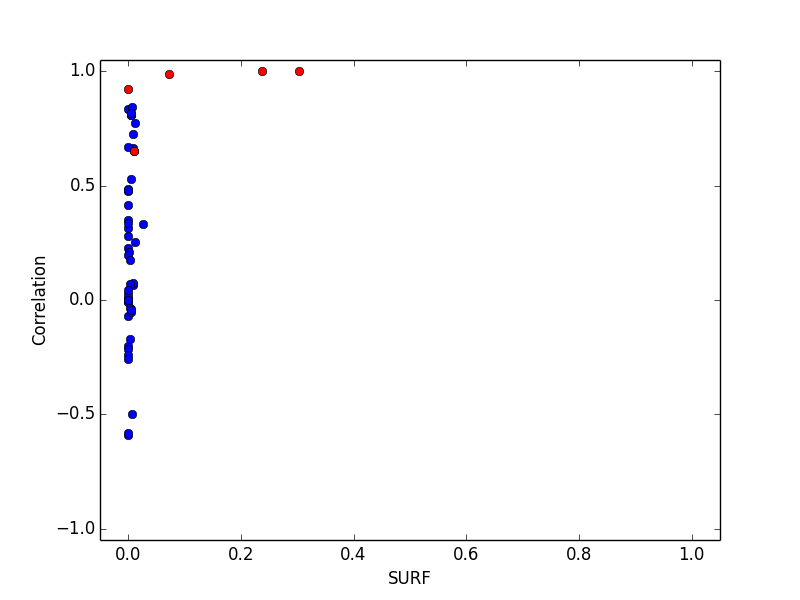
\includegraphics[keepaspectratio,width=1\textwidth]{3}\\
  {News 3}
  \end{center}
\end{subfigure}%
\begin{subfigure}{.25\textwidth}
  \begin{center}
  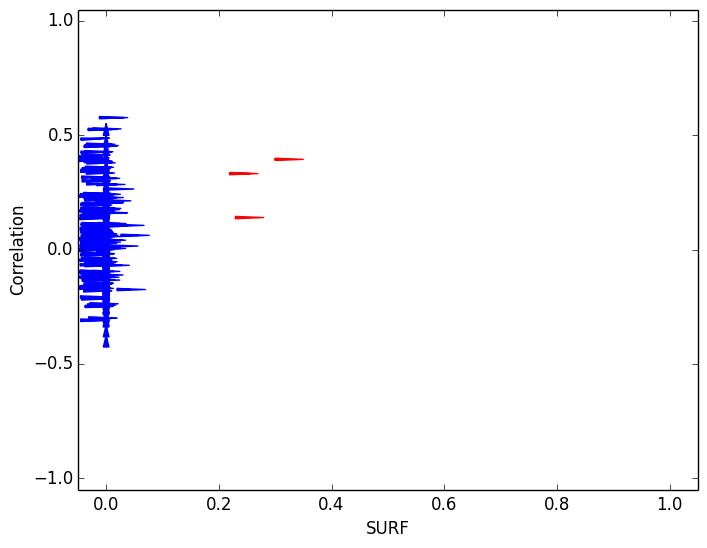
\includegraphics[keepaspectratio,width=1\textwidth]{4}\\
  {News 4}
  \end{center}
\end{subfigure}

\caption{SURF / Correlation}\label{newssurfcorr}
\end{figure}


In the union of all the plot \ref{newssurfcorrgen} we see a really condensed cloud of image in a low SURF measure and in a $[-0.5,0,5]$ correlation interval.\\
Note that there's some similar images that, after a double check with another human-tester, are just been flagged as similar becuase they are \emph{semantically} similar, as we can see in \ref{4simimm}.

\begin{figure}[!ht]
  \begin{center}
  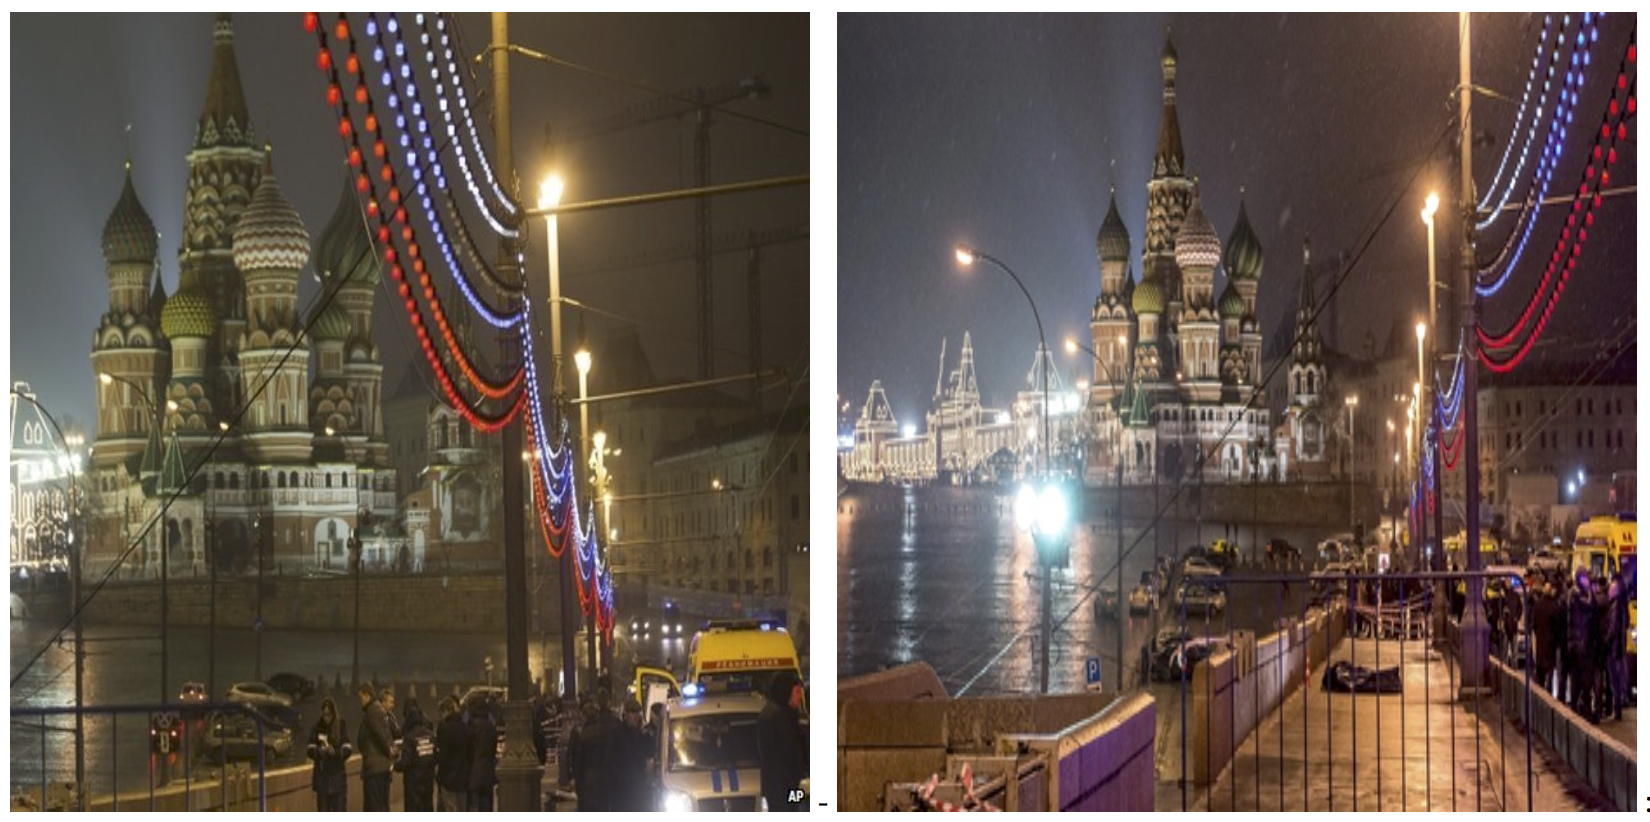
\includegraphics[keepaspectratio,width=0.4\textwidth]{4sim}\\
  \caption{Example of \emph{semantically} similar images}\label{4simimm}
  \end{center}
\end{figure}

Around the central cloud, we have isolated point which are for the majority similar and correct image.

\begin{figure}[!ht]
  \begin{center}
  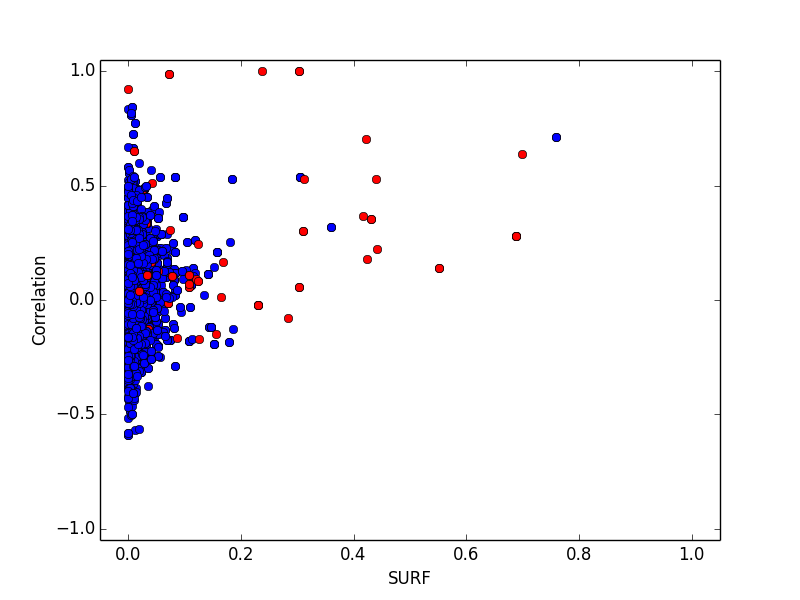
\includegraphics[keepaspectratio,width=0.4\textwidth]{1234}\\
  \caption{General SURF / Correlation}\label{newssurfcorrgen}
  \end{center}
\end{figure}

\textbf{\emph{Farci un elisse intorno alla nuvola e dire che quelle fuori sono simili?}}

After this analisis on the corelation, we focus on the \emph{date}-metadata for the similar images for all the three news.

\begin{figure}[!ht]
\begin{subfigure}{.25\textwidth}
  \begin{center}
  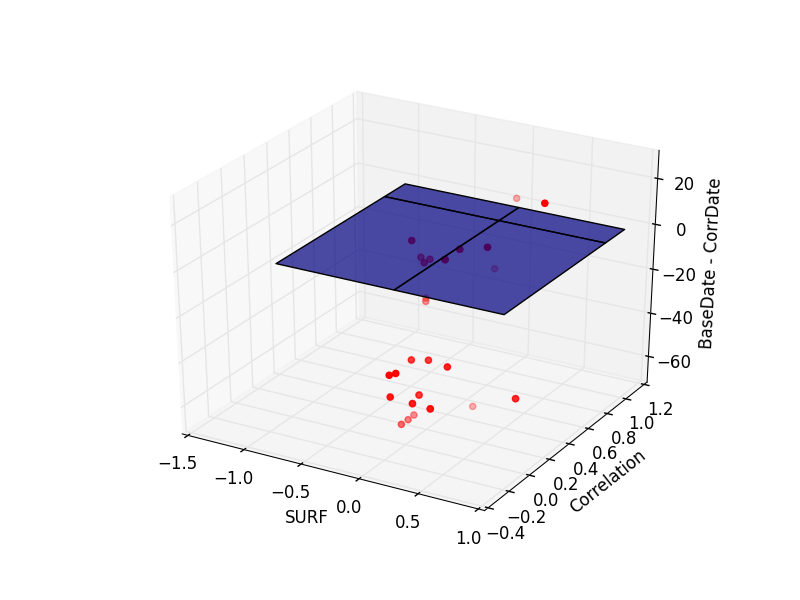
\includegraphics[keepaspectratio,width=1\textwidth]{1234t}\\
  \end{center}
\end{subfigure}%
\begin{subfigure}{.25\textwidth}
  \begin{center}
  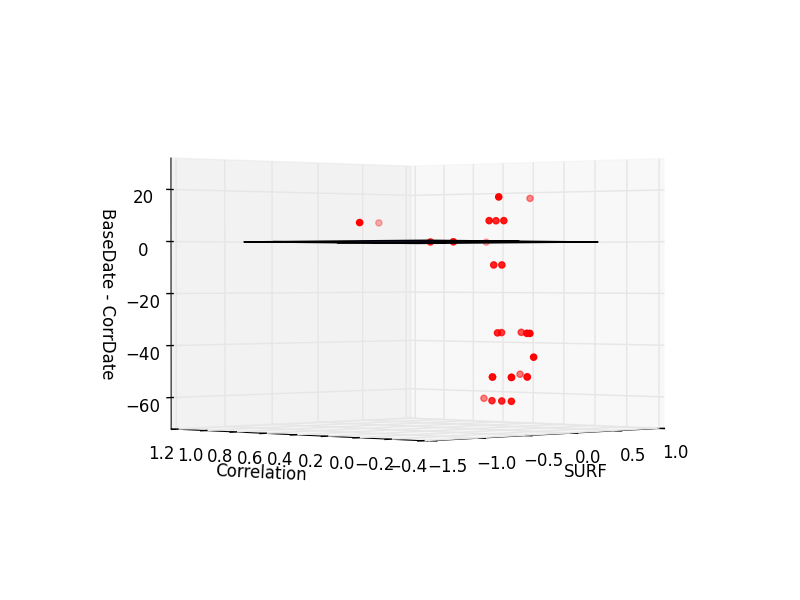
\includegraphics[keepaspectratio,width=1\textwidth]{1234t2}\\
  \end{center}
\end{subfigure}

\caption{SURF / Correlation / Original Date - Correlated Date}\label{datemeta3d}
\end{figure}

From the data we can achieve that some news with similar images have differt \emph{date}-metadata ($0$ means that the date are identical).

\newpage


\subsection{Threshold-like only}


From the statistic obtained by the previous test, we choose as the similarity function
\[ f(\tau_{\text{SURF}} , \tau_{\text{cor}}) = \xi * \xi^{-1} \]

With these schema, we analysed $n$ news :
\begin{enumerate}
  \item link1
  \item $\cdots$
  \item link$n$
\end{enumerate}

\subsection{Human-Threshold check}

Using the previous result, we double-controlled with the two methods:

\begin{enumerate}
  \item link1
  \item link2
\end{enumerate}




% needed in second column of first page if using \IEEEpubid
%\IEEEpubidadjcol


% An example of a floating figure using the graphicx package.
% Note that \label must occur AFTER (or within) \caption.
% For figures, \caption should occur after the \includegraphics.
% Note that IEEEtran v1.7 and later has special internal code that
% is designed to preserve the operation of \label within \caption
% even when the captionsoff option is in effect. However, because
% of issues like this, it may be the safest practice to put all your
% \label just after \caption rather than within \caption{}.
%
% Reminder: the "draftcls" or "draftclsnofoot", not "draft", class
% option should be used if it is desired that the figures are to be
% displayed while in draft mode.
%
%\begin{figure}[!t]
%\centering
%\includegraphics[width=2.5in]{myfigure}
% where an .eps filename suffix will be assumed under latex, 
% and a .pdf suffix will be assumed for pdflatex; or what has been declared
% via \DeclareGraphicsExtensions.
%\caption{Simulation results for the network.}
%\label{fig_sim}
%\end{figure}

% Note that IEEE typically puts floats only at the top, even when this
% results in a large percentage of a column being occupied by floats.


% An example of a double column floating figure using two subfigures.
% (The subfig.sty package must be loaded for this to work.)
% The subfigure \label commands are set within each subfloat command,
% and the \label for the overall figure must come after \caption.
% \hfil is used as a separator to get equal spacing.
% Watch out that the combined width of all the subfigures on a 
% line do not exceed the text width or a line break will occur.
%
%\begin{figure*}[!t]
%\centering
%\subfloat[Case I]{\includegraphics[width=2.5in]{box}%
%\label{fig_first_case}}
%\hfil
%\subfloat[Case II]{\includegraphics[width=2.5in]{box}%
%\label{fig_second_case}}
%\caption{Simulation results for the network.}
%\label{fig_sim}
%\end{figure*}
%
% Note that often IEEE papers with subfigures do not employ subfigure
% captions (using the optional argument to \subfloat[]), but instead will
% reference/describe all of them (a), (b), etc., within the main caption.
% Be aware that for subfig.sty to generate the (a), (b), etc., subfigure
% labels, the optional argument to \subfloat must be present. If a
% subcaption is not desired, just leave its contents blank,
% e.g., \subfloat[].


% An example of a floating table. Note that, for IEEE style tables, the
% \caption command should come BEFORE the table and, given that table
% captions serve much like titles, are usually capitalized except for words
% such as a, an, and, as, at, but, by, for, in, nor, of, on, or, the, to
% and up, which are usually not capitalized unless they are the first or
% last word of the caption. Table text will default to \footnotesize as
% IEEE normally uses this smaller font for tables.
% The \label must come after \caption as always.
%
%\begin{table}[!t]
%% increase table row spacing, adjust to taste
%\renewcommand{\arraystretch}{1.3}
% if using array.sty, it might be a good idea to tweak the value of
% \extrarowheight as needed to properly center the text within the cells
%\caption{An Example of a Table}
%\label{table_example}
%\centering
%% Some packages, such as MDW tools, offer better commands for making tables
%% than the plain LaTeX2e tabular which is used here.
%\begin{tabular}{|c||c|}
%\hline
%One & Two\\
%\hline
%Three & Four\\
%\hline
%\end{tabular}
%\end{table}


% Note that the IEEE does not put floats in the very first column
% - or typically anywhere on the first page for that matter. Also,
% in-text middle ("here") positioning is typically not used, but it
% is allowed and encouraged for Computer Society conferences (but
% not Computer Society journals). Most IEEE journals/conferences use
% top floats exclusively. 
% Note that, LaTeX2e, unlike IEEE journals/conferences, places
% footnotes above bottom floats. This can be corrected via the
% \fnbelowfloat command of the stfloats package.




\section{Conclusion}
The conclusion goes here.





% if have a single appendix:
%\appendix[Proof of the Zonklar Equations]
% or
%\appendix  % for no appendix heading
% do not use \section anymore after \appendix, only \section*
% is possibly needed

% use appendices with more than one appendix
% then use \section to start each appendix
% you must declare a \section before using any
% \subsection or using \label (\appendices by itself
% starts a section numbered zero.)
%


% \appendices
% \section{Proof of the First Zonklar Equation}
% Appendix one text goes here.

% % you can choose not to have a title for an appendix
% % if you want by leaving the argument blank
% \section{}
% Appendix two text goes here.


% % use section* for acknowledgment
% \section*{Acknowledgment}


% The authors would like to thank...


% Can use something like this to put references on a page
% by themselves when using endfloat and the captionsoff option.
\ifCLASSOPTIONcaptionsoff
  \newpage
\fi



% trigger a \newpage just before the given reference
% number - used to balance the columns on the last page
% adjust value as needed - may need to be readjusted if
% the document is modified later
%\IEEEtriggeratref{8}
% The "triggered" command can be changed if desired:
%\IEEEtriggercmd{\enlargethispage{-5in}}

% references section

% can use a bibliography generated by BibTeX as a .bbl file
% BibTeX documentation can be easily obtained at:
% http://www.ctan.org/tex-archive/biblio/bibtex/contrib/doc/
% The IEEEtran BibTeX style support page is at:
% http://www.michaelshell.org/tex/ieeetran/bibtex/
%\bibliographystyle{IEEEtran}
% argument is your BibTeX string definitions and bibliography database(s)
%\bibliography{IEEEabrv,../bib/paper}
%
% <OR> manually copy in the resultant .bbl file
% set second argument of \begin to the number of references
% (used to reserve space for the reference number labels box)
% \begin{thebibliography}{1}

% % \bibitem{IEEEhowto:kopka}
% % H.~Kopka and P.~W. Daly, \emph{A Guide to \LaTeX}, 3rd~ed.\hskip 1em plus
% %   0.5em minus 0.4em\relax Harlow, England: Addison-Wesley, 1999.

% \end{thebibliography}

% biography section
% 
% If you have an EPS/PDF photo (graphicx package needed) extra braces are
% needed around the contents of the optional argument to biography to prevent
% the LaTeX parser from getting confused when it sees the complicated
% \includegraphics command within an optional argument. (You could create
% your own custom macro containing the \includegraphics command to make things
% simpler here.)
%\begin{IEEEbiography}[{\includegraphics[width=1in,height=1.25in,clip,keepaspectratio]{mshell}}]{Michael Shell}
% or if you just want to reserve a space for a photo:

% \begin{IEEEbiography}{Michael Shell}
% Biography text here.
% \end{IEEEbiography}

% % if you will not have a photo at all:
% \begin{IEEEbiographynophoto}{John Doe}
% Biography text here.
% \end{IEEEbiographynophoto}

% % insert where needed to balance the two columns on the last page with
% % biographies
% %\newpage

% \begin{IEEEbiographynophoto}{Jane Doe}
% Biography text here.
% \end{IEEEbiographynophoto}

% You can push biographies down or up by placing
% a \vfill before or after them. The appropriate
% use of \vfill depends on what kind of text is
% on the last page and whether or not the columns
% are being equalized.

%\vfill

% Can be used to pull up biographies so that the bottom of the last one
% is flush with the other column.
%\enlargethispage{-5in}



% that's all folks
\end{document}


